\documentclass[rep.tex]{subfiles}
\begin{document}

\chapter{Zadanie 14}
\label{zad14}
\section{Treść}
Zaprojektować dwusekcyjny, trójwrotowy dzielnik sygnału mikrofalowego obciążony od strony wejścia rezystancją $Z_{01} = 35~\Omega$.
Wrota wyjściowe tego dzielnika są obciążone rezystancjami $Z_{02} = Z_{03} = 50~\Omega$, odpowiednio.
Projekt wykonać, przy założeniu, że środkowa częstotliwość pasma pracy $f_0 = 1.35~GHz$.
Wyznaczyć częstotliwościowe charakterystyki dopasowania we wrotach wejściowych $WFS(f)$ i izolacji (separacji) pomiędzy wrotami $I(f)[dB]$ w paśmie od $f_1 = 1.25~GHz$ do $f_2 = 1.45~GHz$.

\begin{figure}[!htbp]
  \centering
  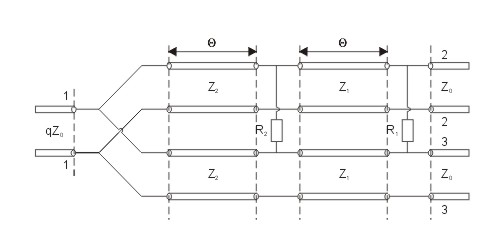
\includegraphics[width=0.5\linewidth]{fig/zad14/div}
  \caption{Schemat elektryczny dzielnika}
  \label{fig:zad14:div}
\end{figure}

\section{Rozwiązanie}
\subsection{Projekt dzielnika}
Projektowany dzielnik jest przedstawiony na rys.~\ref{fig:zad14:div}.
Ze względu na różne impedancje obciążenia i źródła dzielnik musi transformować impedancje.
Przyjmując $Z_0 = 50~\Omega = q \times Z_0$, stąd $q = 0.7$.

Impedancję sekcji dzielnika są opisane zależnościami:
\begin{align}
  Z_1 &= Z_0 \times V_1 \\
  Z_2 &= Z_0 \times V_2
\end{align}
gdzie:
\begin{align}
  V_1^2 &= \sqrt{C^2 + 2q} + C
  V_2   &= \frac{2q}{V_1^2}
  C     &= \frac{(2q - 1) u_0^2}{2(2 - u_0^2)}
  u_0   &= \sin\Big(\frac{w \pi}{4}\Big)
  w     &= \frac{2(f_2 - f_1)}{f_1 + f_2}
\end{align}
Dla danych z treści zadania otrzymuje się:
\begin{align}
  Z_1 &= 54.4190599649~\Omega \nonumber \\
  Z_2 &= 64.3157011947~\Omega \nonumber
\end{align}

Rezystory separujące oblicza się z zależności:
\begin{align}
  R_2 &= \frac{2 Z_1 Z_2}{\sqrt{(Z_1 + Z_2)(Z_2 - Z_1\ctg^2(\theta_3))}} \\
  R_1 &= \frac{2 R_2(Z_1 + Z_2)}{R_2 \frac{Z_1 + Z_2}{Z_0} - 2Z_2}
  \theta_3 &= \frac{ \pi}{2} \Big(1 - \frac{2}{2\sqrt{2}} \Big)
\end{align}
co daje wynik:
\begin{align}
  R_2 &= 80.3347745707~\Omega \nonumber \\
  R_1 &= 307.005233567~\Omega \nonumber
\end{align}

\subsection{Charakterystyki dzielnika}
W celu wyznaczenia charakterystyki częstotliwościowej dopasowania we wrotach wejściowych:
\begin{equation}
  WFS(f) = \frac{1 + |S_{11}|}{1 - |S_{11}|} \label{eqn:zad14:wfs}
\end{equation}
Izolację z kolei określa zależność:
\begin{equation}
  I(f) = 20 \log \Big( \frac{1}{|S_{23}|} \Big) \label{eqn:zad14:I}
\end{equation}

Niezbędne parametry macierzy rozproszenia S:
\begin{align}
  S_{11} &= \frac{-RN + jXN}{RD + jXD} \\
  S_{23} &= \frac{1}{2} \bigg[\frac{RN + jXN}{RD + jXD} - S_{22}^{+-}\bigg] \\
  S_{22}^{+-} &= \frac{A + jB}{C + jD} \\
\end{align}
Dokładne zależności podane zostały w~\cite{obwody}.
Charakterystyki dzielnika zaprezentowano na rys.~\ref{fig:zad14:iso}~i~\ref{fig:zad14:wfs}.

\begin{figure}[!htbp]
  \centering
  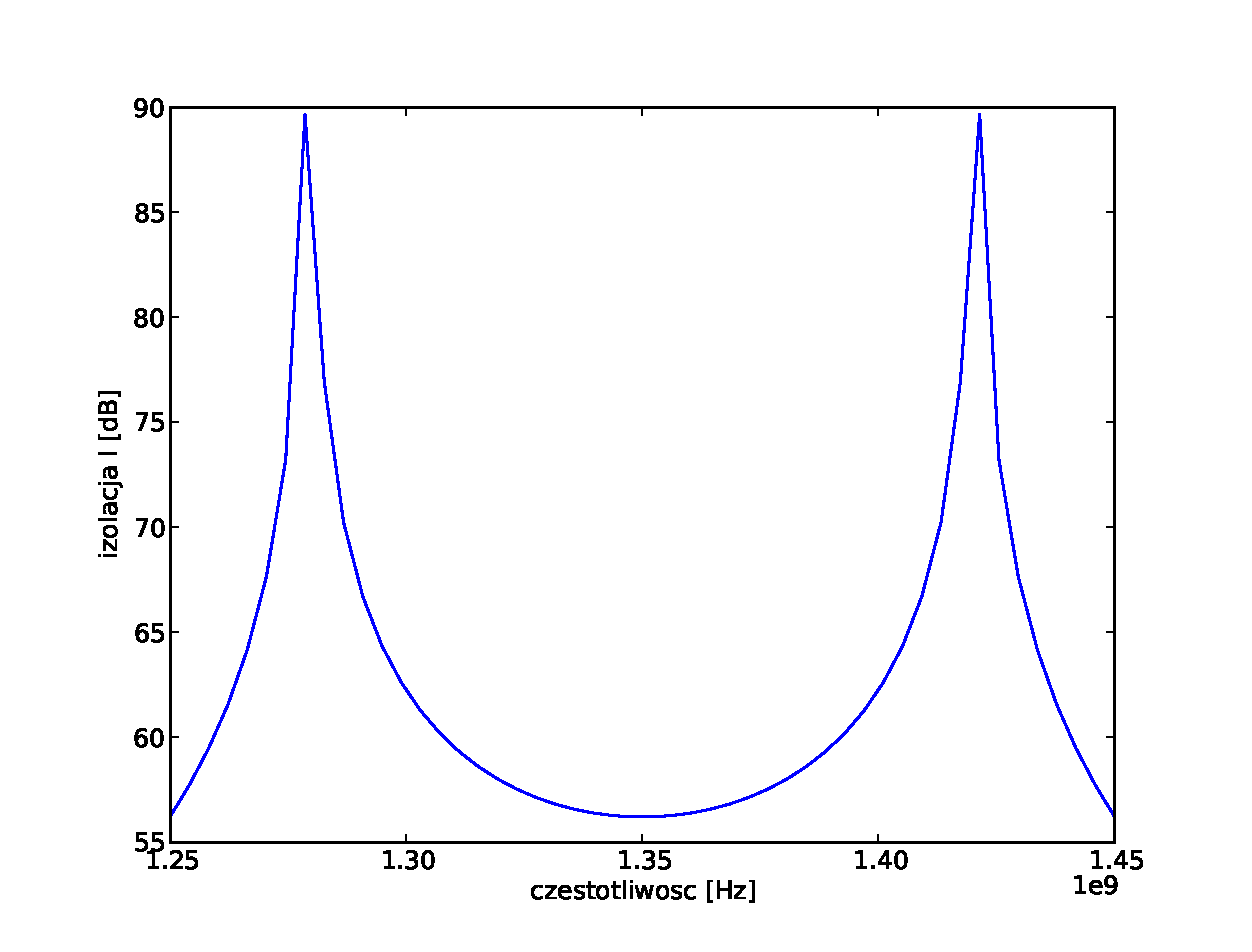
\includegraphics[scale=0.5]{fig/zad14/iso}
  \caption{Charakterystyka izolacji dzielnika}
  \label{fig:zad14:iso}
\end{figure}

\begin{figure}[!htbp]
  \centering
  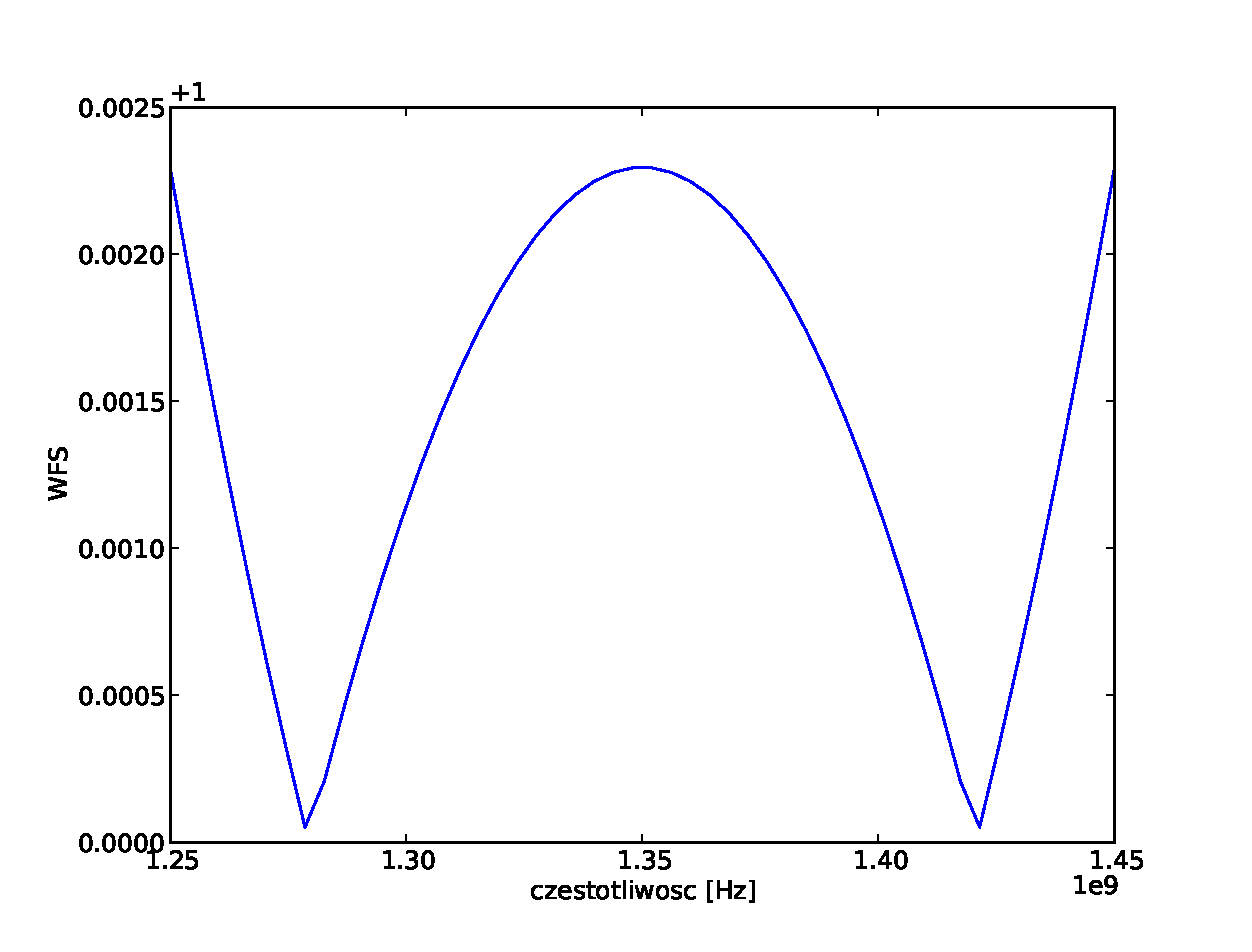
\includegraphics[scale=0.5]{fig/zad14/wfs}
  \caption{WFS na wejściu dzielnika}
  \label{fig:zad14:wfs}
\end{figure}

\end{document}
